\subsection{User Cycle}\label{sec:ladeablauf}

Um einen lückenlosen Betrieb zu gewährleisten, ist ein Ablauf für den Gebrauch des Dojos notwendig. Dieser Ablauf wird in vier Schritte unterteilt und ist in Abbildung \ref{fig:Ladezyklus Dojo} ersichtlich.
Die Betriebszeit des Dojos ermöglicht eine Betriebszeit von fünf Stunden, wobei durch Ladezyklen zwischen den Besuchen eine ganztägiger Betrieb ermöglicht wird. Darum wurde im Ziel 5.1 ein Arbeitstag genannt. Um dies zu veranschaulichen, gibt nachfolgende Abbildung \ref{fig:Ladezyklus Dojo} einen Einblick ins Konzept.

\begin{figure}[H]
	\begin{center}
		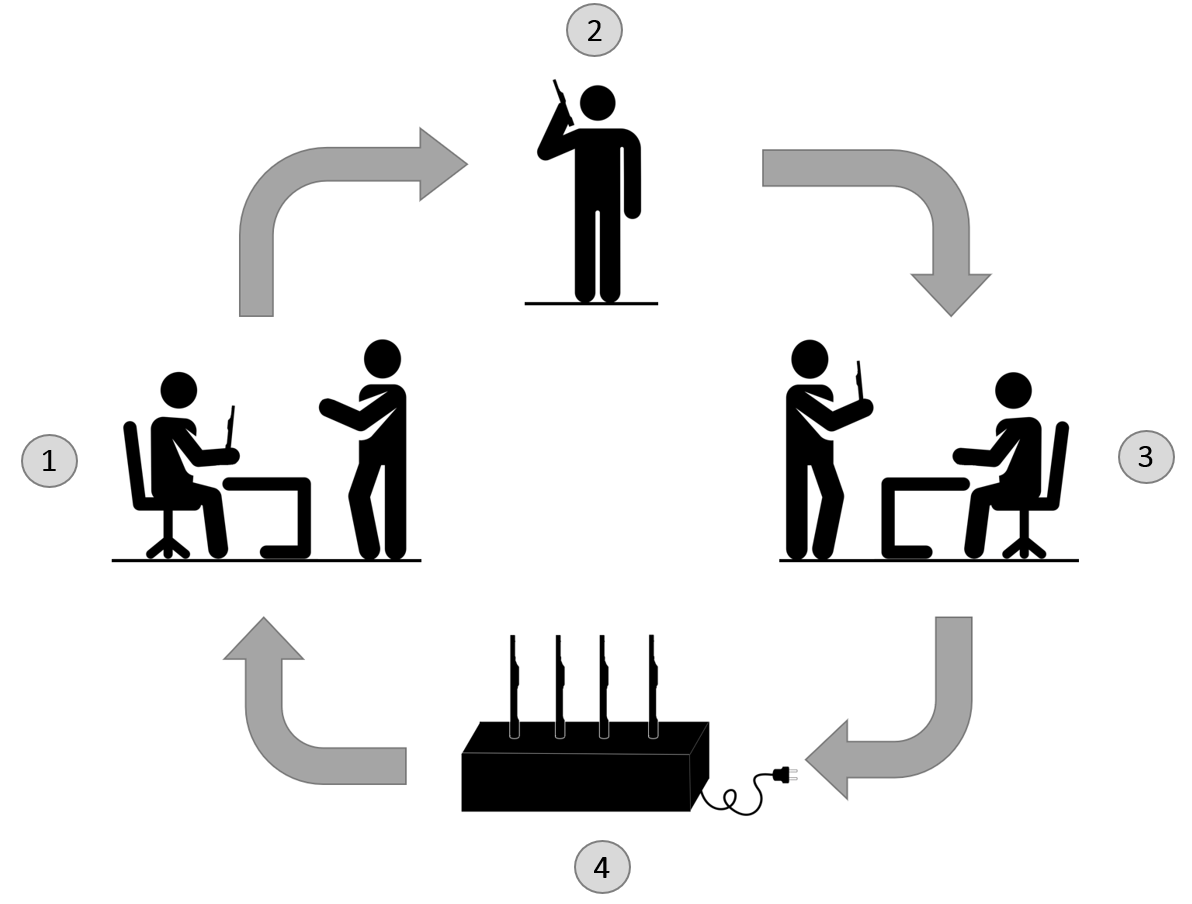
\includegraphics[width=140mm]{data/Ladezyklus.png}
		\caption[User Cycle Dojo]{User Cycle Dojo} %picture caption
		\label{fig:Ladezyklus Dojo}
	\end{center}
\end{figure}

Der erste Schritt beinhaltet die Dojo Ausgabe beim Empfang. Hierbei wird bereits festgelegt welche Sprache verwendet und in welche Bereiche der Besucher Zutritt erhalten soll. Diese Einstellungen können von Besucher zu Besucher variieren. Zu beachten gilt es, dass jeweils die Geräte ausgegeben werden, welche sich am längsten in der Ladestation (Schritt 4) befinden. Bei einer Stückzahl welche grösser ist als die Besucherzahl, erlaubt dies einen lückenlosen Betrieb.
\\
\\
In Schritt 2 befindet sich der Besucher auf dem Rundgang mit dem Dojo als Audio-Guide. Der Nutzer hat hierbei die Möglichkeit während dem Rundgang Bilder zu \glqq liken\grqq . Weitere Funktionen und die Bedienung des Dojos selber, ist im vorherigen Unterkapitel \ref{sec:funktionsweise} beschrieben.
\\
\\
Die Abgabe erfolgt in Schritt 3. Hier hat der Besucher die Möglichkeit \glqq gelikte\grqq Bilder als Broschüre zu erhalten oder diese per Mail zu erhalten. Das entgegengenommene Dojo kann für den nächsten Besucher gereinigt werden.
\\
\\
Sobald das Dojo entgegengenommen wurde und alle benötigten Informationen (\glqq likes\grqq) extrahiert wurden, wird es wie in Schritt 4 ersichtlich aufgeladen. Hierfür ist eine Ladestation verfügbar, wobei es lediglich notwendig ist die Dojos in die dafür vorgesehenen Ladebuchsen zustecken. Hierbei beginnt der induktive Ladezyklus sobald die in jedem Gerät eingebaute Signal-LED zu leuchten beginnt.
